\documentclass[Visionprosjekt.tex]{subfiles}
\NormalTopp
\begin{document}

%%%%%%%%%%%%%%%%%%%%%%%%%%%%%%%%%%%%%%%%%%%%%%%%
\section{Vision}
%%%%%%%%%%%%%%%%%%%%%%%%%%%%%%%%%%%%%%%%%%%%%%%%

Begrepet «vision» innen for automasjonsindustrien kan deles inn i tre hovedgrupper:

\begin{description}[style=multiline,leftmargin=32mm]
	\item[Vision-sensor] En vision-sensor er den «dummeste» typen vision-produkt. Den har inne\-bygd bildebehandlingsenhet i kamerahuset. Enheten arbeider etter forhåndsprogrammerte regler, og gir ofte bare binære utgangsverdier.  Det er denne typen vision som er brukt i dette prosjektet.

     \item[Vision-kamera] Et vision-kamera har mulighet for mer datautveksling, f.eks. over en feltbuss. Kameraet kan gjøre mer avanserte avlesninger og bildebehandlinger, som f.eks. strekkodelesing og tekstgjenkjenning.

     \item[Vision-system] Hvis  mange vision-kameraer «samarbeider», kan dette kalles et vision-system. Dette er den mest avanserte typen vision-produkt.
\end{description}

I denne rapporten   beholdes den daglige talemåten «vision-kamera», selv om  enheten i dette anlegget  strengt tatt er en vision-sensor.

Uansett hvilken vision-enhet som velges, vil en viktig del være det digitale kameraet. I sin enkleste form består et digitalt kamera av et objektiv, en bildebrikke, en rådata bildebehandler, og en lystett kapsling. Bildebrikken har flere tusen små, lysfølsomme punkter, kalt piksler. Objektivet vil,  tegne et bilde på bildebrikka når  fokusen er korrekt justert. \refF{fig:kamera} illustrerer hvordan kameraet er bygd opp. I kameraet som er brukt i dette prosjektet, vil hvert enkelt punkt på bildebrikken overføre en verdi mellom 0 og 255 som forteller hvor sterk lysintensiteten er på  punktet. Verdiene blir normalisert til verdier mellom 0 og 100 i bildebehandlingsdelen. \cite{framework}

\begin{figure}[ht]
	\centering
		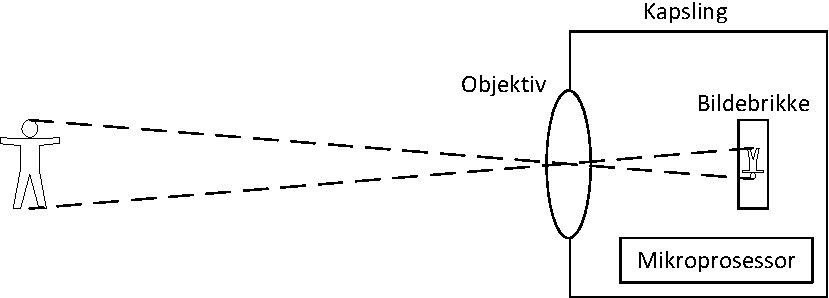
\includegraphics{bilder/kamera}
	\caption{Virkemåten til et kamera}
    \label{fig:kamera}
\end{figure}

Videre vil dette kapitlet beskrive kameraet som er benyttet  i prosjektet, strekkodestandarden «Data Matrix» og  hvordan kameraet er konfigurert for kunne å lese disse.






%%%%%%%%%%%%%%%%%%%%%%%%%%%%%%%%
\subsection{DVT Legend 530}
%%%%%%%%%%%%%%%%%%%%%%%%%%%%%%%%
I transportbåndmodellen er kameraet DVT Legend 530, sammen med en I/O-modul for kommunikasjon med PLS, benyttet. Kameraet inneholder  bildeanalysatoren  "<\mbox{SmartImage} \mbox{Sensor}">. Det er bildeanalysatoren som er selve hjernen til kameraet, den analyserer bildet etter forhåndsdefinerte regler.



 Kommunikasjon mellom PC og kamera går over Ethernet 100BASE-TX. Se \reft{tab:legend530} for spesifikasjoner for kameraet DVT Legend 530 \cite{dvtlegend530}.

\begin{table}[ht]
    \centering
    \caption{Spesifikasjoner for DVT Legend 530}
    \label{tab:legend530}
    \begin{tabular}{ll}
    \toprule
        Egenskap        &   Verdi\\
    \midrule
        Bildebrikke	    &	4.8\,mm $\times$ 3.6\,mm CCD\\
        Oppløsning	    &	640\,px $\times$ 480\,px gråskala\\
        Strømtilførsel	&	24\,VDC 210 mA\\
        Temperaturområde i drift	&	0--45\,°C\\
        Objektivfeste	&	CS-feste\\
        Ekstrautstyr	&	LED-belysning\\
        \bottomrule
    \end{tabular}
\end{table}







%%%%%%%%%%%%%%%%%%%%%%%%%%%%%%%%
\subsubsection{Valg og tilpasning av objektiv}
%%%%%%%%%%%%%%%%%%%%%%%%%%%%%%%%


Det er tilgang på to objektiver for kameraet, hvor hovedforskjellen er fokuslengden. Se \reft{tab:objektiver} for spesifikasjoner for de to objektivene.



\begin{table}[ht]
    \centering
    \caption{Spesifikasjoner for objektivene}
    \label{tab:objektiver}
    \begin{tabularx}{0.70\textwidth}{llX}
        \toprule
         Egenskap               &	6\,mm f/1.4	&	 Tamron 16\,mm f/1.4\\
        \midrule
        Feste	                &	C-feste	    &	C-feste\\
        Fokuslengde	            &	6\,mm	    &	16\,mm\\
        Største blenderåpning	&	f/1.4	    &	f/1.4\\
        Minste blenderåpning	&	Stengt	    &	f/16\\
        Nærgrense	            &	20\,cm	    &	30\,cm\\
        \bottomrule
    \end{tabularx}
\end{table}


CS-festet på kameraet har en FFD på 12,526\,mm, mens C-festet på objektivene har en FFD på 17,526\,mm \cite{CSmount}. For å få riktig FFD, er det satt inn en 5\,mm fokusforlenger. Utprøving av kameraet og objektivene viste at fokusforlengeren ikke fungerte tilfredsstillende, bildet ble uskarpt. Derfor er det laget en 1\,mm tykk skive som flytter FFD ned til 18,526\,mm.
Med denne skiven ble også nærgrensen  til objektivet  lavere, som betyr at kameraet må settes nærmere objektene som skal fotograferes.


Det er valgt en avstand mellom kamera og objekt på 180\,mm. Ved den avstanden må objektivets fokus stilles på  0,33\,m for å få et skarpt bilde. Blenderåpningen er stilt inn på f/4.





%%%%%%%%%%%%%%%%%%%%%%%%%%%%%%%%%%%%
\subsection{Datamatriser}
%%%%%%%%%%%%%%%%%%%%%%%%%%%%%%%%%%%%

Datamatriser er todimensjonale strekkoder bestående av en samling moduler/celler som kan innta to tilstander -- svart eller hvit i dette tilfellet. Datamatriser kan inneholde betydelig mer informasjon enn strekkoder på grunn av den ekstra dimensjonen med informasjon.
%Det må benyttes et kamera for å  lese en datamatrise, noe som gjør datamatriser egnet til å identifisere beholderene.
Datamatriser defineres av standarden ISO/IEC 16022:2006  \cite{iso16022}.

En datamatrise er satt sammen  av et L-formet "<Finder pattern">, et "<Timing pattern">, og selve datainnholdet. Rundt datamatrisen må det være en "<Quiet zone"> i alle retninger, minst en modul-/cellestørrelse bred/lang. \cite{iso16022}

Størrelsen på en datamatrise varierer fra $10\times10$ til $144\times144$ celler, og kan romme fra 1\,byte (3\,alfanumeriske tegn) til 1556\,byte (2335\,alfanumeriske tegn) med data \cite{IDautomation}. \refF{fig:datamatrise} viser oppbygningen av en $16\times16$-datamatrise som kan romme 10\,byte med datainnhold.


\begin{figure}[ht]
	\centering
		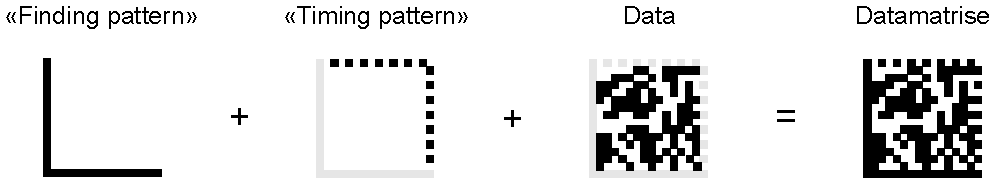
\includegraphics[scale=1]{bilder/datamatrise.pdf}
	\caption{Oppbygning av en $16\times16$-datamatrise}
	\label{fig:datamatrise}
\end{figure}


I dette prosjektet er det benyttet tre forskjellige $16\times16$-datamatriser, generert ved hjelp av web-verktøyet \cite{DataMartixGenerator}. Innholdet i matrisene er tekstene "<Produkt 1">, "<Produkt 2"> og "<Produkt 3">. \refF{fig:datamatriser} viser disse datamatrisene.

\begin{figure}
	\centering
		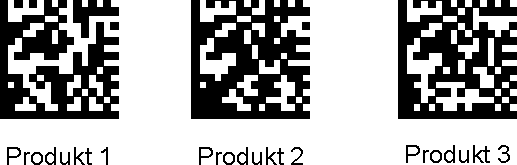
\includegraphics[scale=1]{bilder/datamatriser.pdf}
	\caption{Datamatriser som inneholder tekstene "<Produkt 1">, "<Produkt 2"> og "<Produkt 3">}
	\label{fig:datamatriser}
\end{figure}










%%%%%%%%%%%%%%
\subsubsection{Plassering av datamatriser på bokser}
%%%%%%%%%%%%%%

Datamatrisene er skrevet ut i størrelse $9\times9$\,mm, tilsvarende 20 moduler per cm (dette inkluderer "<Quiet-zone">). På grunn av den lille størrelsen må plasseringen av datamatrisene på boksene være nokså presis.
Det fotograferte området kun 14\,mm høyt, se underkapittel \ref{subsection(Konfigurering-av-visionkamera)}.
  Dette betyr at  toleransen for plassering av matrisen i høyderetningen er $\pm$2,5\,mm. Datamatrisene må derfor plasseres \emph{nøyaktig} i henhold til \reff{fig:plasseringdatamatrise}.


% \red{Rart at det ikke nevnes \emph{noe} om lengderetningen!}

\begin{figure}
	\centering
		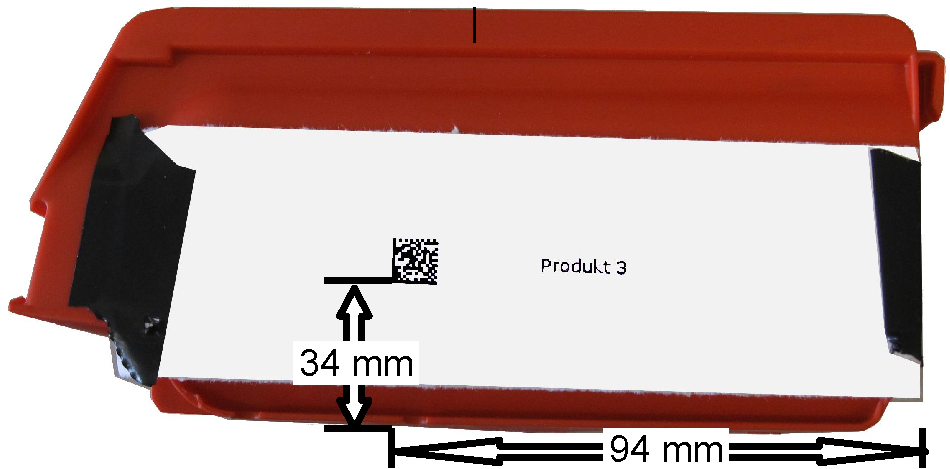
\includegraphics[width=0.8\textwidth]{bilder/plasseringdatamatrise.pdf}
	\caption{Retningslinjer for plassering av datamatrise på beholder}
	\label{fig:plasseringdatamatrise}
\end{figure}












%%%%%%%%%%%%%%%%%%%%%%%%%%%%%%%%%%%%%%%%%%%%%
\subsection{Konfigurering av visionkamera}\label{subsection(Konfigurering-av-visionkamera)}
%%%%%%%%%%%%%%%%%%%%%%%%%%%%%%%%%%%%%%%%%%%%%
Før vision-kameraet kan lese datamatriser, må det konfigureres/programmeres. Dette underkapitlet vil beskrive konfigurasjonsprosessen.

På bildeanalysatoren kjører et program, kalt «firmware». Dette programmet må ha samme versjonsnummer som programmeringsverktøyet "<DVT \mbox{FrameWork}"> på datamaskinen.
DVT \mbox{FrameWork}  lastes ned fra produsentens hjemmesider, og inneholder firmware-filer for forskjellige DVT Legend-kameraer. Siste programvareversjon som er fullkompatibelt med DVT Legend 530 er "<DVT \mbox{FrameWork} \mbox{Firmware}  2.8.0">, datert 06.06.2007\footnote{Selv siste versjon av programmet er  utdatert og  ikke fullt kompatibelt med Windows\,Vista elle Windows\,7. Blant annet fungerer ikke firmwareoppgradering og automatisk søk etter vision-kameraet i nettverket.  Dersom DVT Legend 530 skal benyttes i fremtidige prosjekter, bør altså en eldre PC med Windows XP være tilgjengelig.}.


%Visionkameraets firmware ble  oppgradert til FrameWork 2.8.0. Dette gjøres ved å velg "<Load Firmware"> fra oppstartsvinduet som fremkommer når man starter programmeringsverktøyet. Videre velges  filen "<FWK280.530">, som henviser til DVT Legend 530.

Hovedoppgaven til et vision-kamera er å inspisere produkter. Dette kommer også tydelig fram i programmeringsmulighetene til kameraet. Programmet kan settes opp til å inneholde mange "<produkter">, men essensen er ikke at programmet skal gjenkjenne produktet. Et visionkamera vil på forhånd vite hvilket produkt det tar bilde av, og  kun kontrollere dette for visuelle svakheter eller defekter. Er produktet OK, vil kameraet returnere verdien «PASS». Dersom produktet ikke er i orden, returneres verdien «FAIL». Verdiene PASS og FAIL gjøres om til henholdsvis digital 1 og digital 0 i kamaraets I/O-tilkobling. \cite{framework}

Siden dette prosjektet har tre ulike produkter, er det satt opp tre datamatrise-«sensorer» i DVT FrameWork. Sensorene leter i rektangelet fra pikselpunkt $(0,170)$ til $(639,330)$, som tilsvarer et område på rundt $50\times14$\,mm når kameraet er korrekt justert.
Området er valgt så bredt som mulig for å hindre at ulike responstider i PLS-en skal virke inn på bildet.
Et typisk bilde tatt av vision-kameraet er vist i \reff{fig:visionbilde}. Rektanglet markerer området hvor vision-kameraet leter etter datamatriser. Bildet er redigert for å forbedre svart/hvitt-utskrift.

\begin{figure}[ht]
	\centering
		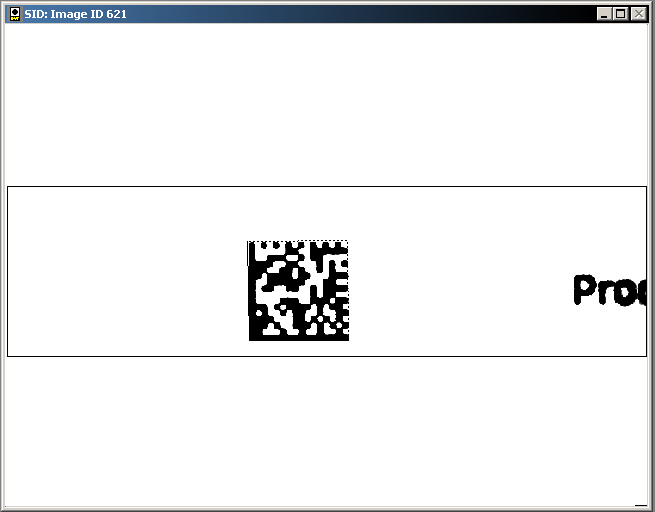
\includegraphics[width=0.618\textwidth]{bilder/visionbilde.png}
	\caption{Typisk bilde tatt av visionkameraet}
    \label{fig:visionbilde}
\end{figure}



Hver sensor vil inspisere bildet og se etter datamatrisen, og returnere PASS eller FAIL. Kriteriet for at en sensor skal returnere PASS er at datamatrisen må finnes, og at det 9. tegnet i datamatrisens datainnhold må samsvare med produktnummeret. Produktnummeret kan  enten være 1, 2 eller 3, og det 9. tegnet vil også være 1, 2 eller 3. Ved  gjenkjent produkt vil altså én av sensorene returnere  PASS, mens resten returnerer FAIL. Dersom datamatrisen ikke kan leses, vil alle sensorene returnere  FAIL.

Dette er den beste måten å programmere DVT Legend 530 til å være en datamatriseleser, men metoden er ressurskrevende. \refF{fig:prosesseringstidx1} viser at gjennomsnittlig prosesseringstid for én sensor er 74\,ms. \refF{fig:prosesseringstidx3} viser at gjennomsnittlig prosesseringstid for tre sensorer er 191 ms. Visionkameraet bruker omlag tre ganger lengre tid enn det som burde være nødvendig i utgangspunktet. Dette viser at vision-kameraet egner seg best til å inspisere, ikke gjenkjenne forskjellige produkter.

\begin{figure}[ht]
	\centering
		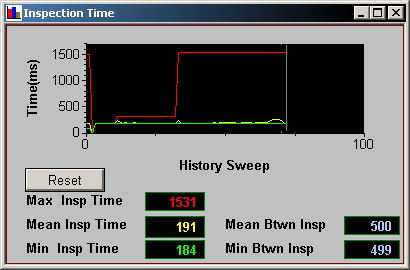
\includegraphics[width=0.618\textwidth]{bilder/prosesseringstidx3.png}
	\caption{Prosesseringstid for én datamatrise-sensor}
    \label{fig:prosesseringstidx1}
\end{figure}


\begin{figure}[ht]
	\centering
		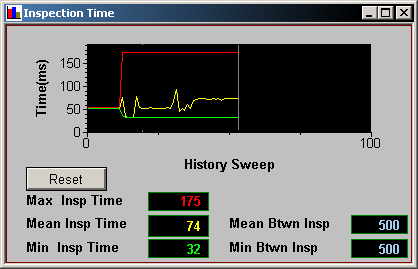
\includegraphics[width=0.618\textwidth]{bilder/prosesseringstidx1.png}
	\caption{Prosesseringstid for tre datamatrise-sensorer}
    \label{fig:prosesseringstidx3}
\end{figure}












\clearpage
%%%%%%%%%%%%%%%%%%%%%%%%%%%%%%%%%%%%%%%%%%%%%%%%%%%
\subsubsection{Oppsett av I/O-parametre i kameraet}
%%%%%%%%%%%%%%%%%%%%%%%%%%%%%%%%%%%%%%%%%%%%%%%%%%%

Visionkameraet har 8 digitale I/O-tilkoplinger. Funksjonen til I/O-tilkoplingene velges i DVT FrameWork. \refT{tab:visionio} viser hvilke funksjoner som er valgt til I/O-tilkoblingene. De brukerdefinerte utgangene \texttt{Out-User1}, \texttt{Out-User2} og \texttt{Out-User3} er programmert slik at \texttt{Out-UserX} vil gå aktiv dersom datamatrisesensoren for produkt \texttt{X} returnerer  PASS. Utgangene vil være aktive i 300\,ms. \refF{fig:iokonfig} viser hvordan I/O-konfigurasjonene er gjort på datamakinen.


\begin{table}[ht]
    \centering
    \caption{I/O-tilkoplingene til visionkameraet}
    \label{tab:visionio}
    \begin{tabular}{l>{\ttfamily}ll}
        \toprule
        Pin &	\normalfont Funksjonsvalg &		Beskrivelse\\
        \midrule
		1 &		Out-User1 &		Brukerdefinert utgang\\
		2 &		Out-User2 &		Brukerdefinert utgang\\
		3 &		Out-User3 &		Brukerdefinert utgang\\
		4 &		(None) &		\\
		5 &		(None) &		\\
		6 &		(None) &		\\
		7 &		Out-Busy &		Aktiv når kameraet behandler siste bilde\\
		8 &		In-Trigger &	Inngang som trigger kameraet til å ta bilde\\
        \bottomrule
    \end{tabular}
\end{table}

\begin{figure}[ht]
	\centering
		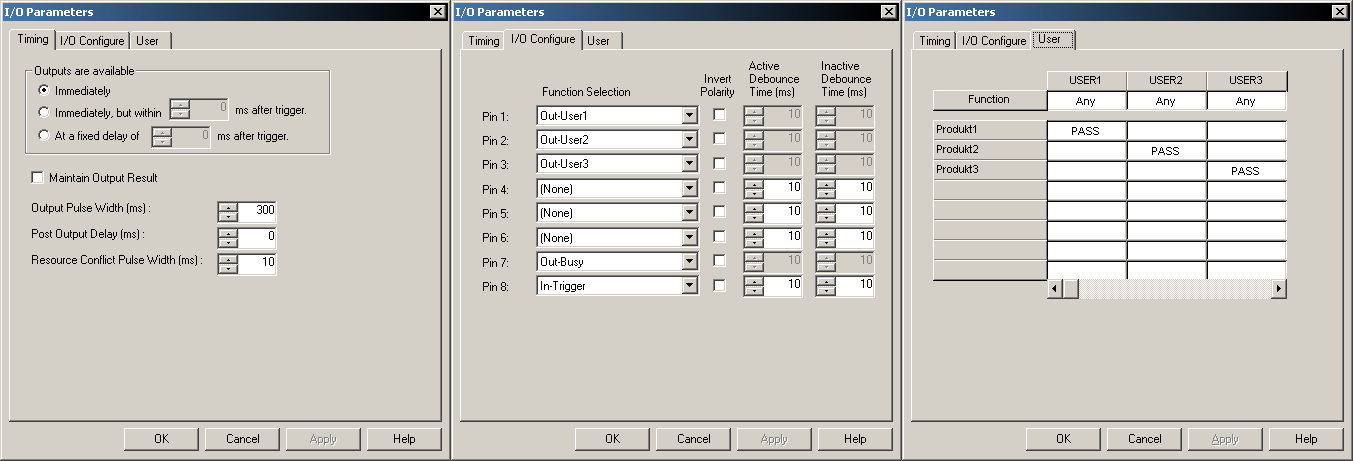
\includegraphics[width=\textwidth]{bilder/iokonfig.png}
	\caption{Skjermdump av I/O-konfigurering til visionkameraet}
    \label{fig:iokonfig}
\end{figure}



\end{document}
